\chapter{绪论}
\section{研究背景和意义}
在过去几年中,世界见证了以Facebook,Twitter,以及国内新浪微博、人人网为代表的社交网络的崛起。Facebook全球已经有超过10亿用户,新浪微博全球注册用户已经达到6亿。据报道,在美国,人们16\%的上网时间停留在Facebook上,超过了传统搜索引擎Google的10\%。社交媒体中保存了大量的用户资料,用户间的社交关系以及海量文本信息,对大数据时代的到来有着不可磨灭的贡献,有着巨大的研究价值,在广告和推荐系统方面,也有着广阔的商业应用前景。

\begin{figure}[!h]
\centering
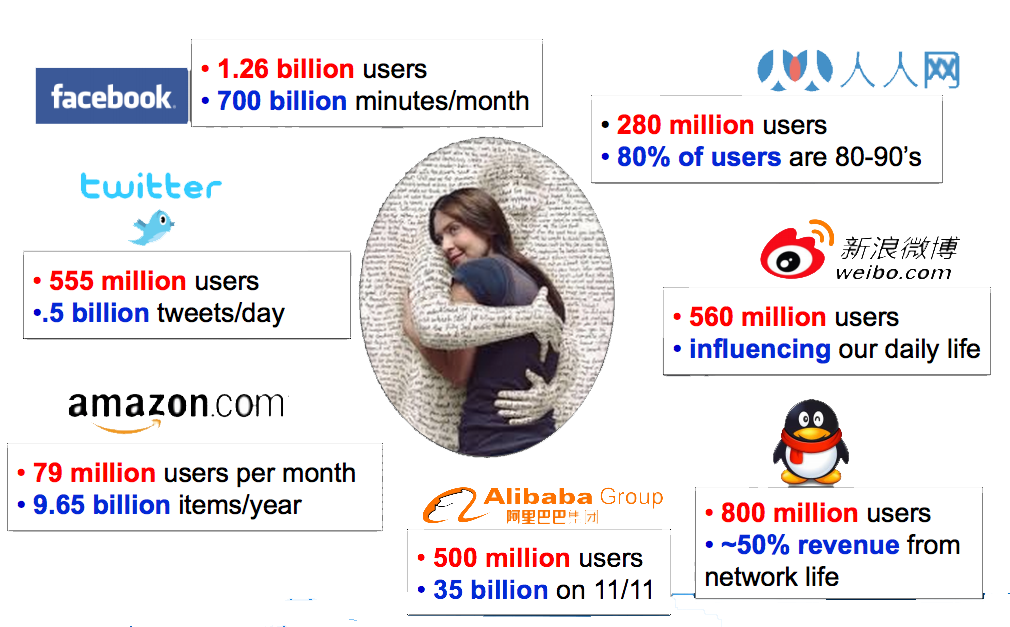
\includegraphics[width=0.8\textwidth]{social_pros.png}
\caption{社交网络的崛起}
\end{figure}

社交网络最初为用户提供了一个信息传播,结识好友的社交平台,用户发布的信息也通常是交流、沟通以及对社会事件的看法。现有的社交网络研究,如网络结构和演化分析\cite{leskovec2008microscopic}, 链接预测\cite{liben2007link}, 影响力分析\cite{tang2009social}, 社会纽带关系推断\cite{tang2011learning}等,更多地考虑社交网络本身的特性和用户的线上行为。而随着移动的互联网的迅猛发展和智能移动通信工具的普及,用户访问社交网络不再局限于传统的个人计算机。朋友聚会,家庭出游等活动中,经常许多人到达目的地的第一件事是拿出手机,在微博或Foursquare等社交网络上签到,告诉朋友们自己现在在做什么,心情如何,社交网络和线下的日常生活以前所未有的方式深入地结合在一起。这也促使我们关注这样一个问题,是否可以从社交媒体的海量数据中挖掘出人们日常活动中的一些知识,比如一项活动通常在什么时间、什么地点发生,两个活动是否存在联系,用户在进行A活动后,最可能去做的下一件事是什么。最终将我们得到的数据进行整理、分析,并实现一个可视化的系统,方便进一步的分析和应用。

相比于其他的Web数据,如点评、论坛、百科、问答平台,社交媒体有不可替代的优势。大众点评、Yelp等点评类网站,同样可以挖掘用户的活动信息,但它以商家为中心,局限于用户消费行为,如就餐、住宿、电影,收集的只是用户对于商家的点评信息。而用户的日常活动,如散步、睡觉等等,用户是不会发布在这些平台上的。用户在类似微博、人人网的社交媒体上,更愿意发布私人化、生活化的内容;同时,得益于移动互联网,用户通过随时随地方便地访问社交平台,获取信息的实时性更好,也更容易获取用户精确的地理信息。同时,社交网络的好友机制,可以帮助我们推断用户在活动中的互动。例如,用户A在时刻$t$发布了一条活动信息的微博并提到了用户B,或者B在相近的地点进行了签到,我们可以推测,B参加了A提到的那一项活动,即使B并没有特意发微博表明这一事实。

对社交网络中活动信息的挖掘,可以预想,有许多潜在的应用,尤其是在推荐系统的应用。
\begin{enumerate}
\item{\heiti 用户行为模式建模} 给定用户$t_0$时刻前的活动历史$history = \{a_t|t<t_0\}$,预测用户在下一时刻$t_0+1$在地点$p$进行活动$a$的概率,即预测$P(p_i, a_j|t+1,history)$。
\item{\heiti 基于兴趣的好友推荐} 现有的社交平台,如Facebook, 人人网等的好友推荐,主要对用户是否认识进行链接预测;而微博的推荐关注,则考虑到被推荐用户的影响力,以及和用户选定兴趣标签的匹配程度。如果我们能对用户参加活动的类别和地点有足够多的了解,就能更精确地向用户推荐兴趣相投的朋友,并且更容易转化为线下的好友关系。
\item{\heiti 个性化的活动推荐} 当用户来到一个陌生的城市,或是有闲暇的时间而不知道如何休闲娱乐,我们可以基于活动的知识,向其推荐活动。比如,一个用户经常在微博中发布吃火锅类似的信息,那么,如果用户来北京旅游,就可以向其推荐东来顺等有特色的涮肉火锅,这也会产生潜在的商业价值。
\end{enumerate}

\section{研究问题与挑战}

本文目标在于建立一个关于社交媒体中活动的系统ActivityNet,并实现以下功能

\begin{enumerate}
\item 对于用户的查询,呈现该活动的相关知识,如活动的类别,地域、时间分布,类似活动等等。
\item 对于特定的社交网络用户(本文工作主要基于新浪微博),分析其活动偏好。
\item 对于给定的地点,推荐当地最热门的活动。
\end{enumerate}

在系统构建过程中,我们需要解决以下问题:

\begin{enumerate}
\item 如何从社交媒体中抽取活动的抽象概念表示。
\item 如何对一条用户发布的信息,构建活动的实例。包括活动概念,情感、地点、时间等相关属性。
\item 如何建模活动之间的关系。我们希望构建一个层次结构,活动之间的关系有不同的类型,例如``A is-a B'',表示B是A概念的外延(如``吃早饭''和``吃饭'');``A follows B''表示A常在B之后依次进行。
\item 如何对得到的知识进行高效地存贮、检索和可视化。
\end{enumerate}

虽然社交媒体相比其他Web数据有诸多优势,其本身的特点也给我们的工作提出了许多挑战:

\begin{enumerate}
\item 问答、论坛等Web平台,其自身的分类系统限定了话题,人们谈论的内容比较单一。而社交媒体中,人们谈论的话题不收限制,可以对自己感兴趣的任何问题发表观点,不仅仅局限在日常活动,不可避免了噪声和稀疏性问题。同时,人们在社交媒体上发布的消息格式高度自由,长度很短,同时常带有俚语和语法、词法的错误。这对信息的精确抽取带来挑战。
\item 社交媒体中对消息长度有严格限制,传统的基于统计的方法不易应用于挖掘活动之间的概念联系。
\item 利用社交网络的结构信息,如好友关系,对未明确表达的参与关系进行推断。
\end{enumerate}

在本文中,主要解决前两个挑战。对隐式的活动参与进行推断有比较大的难度,同时也不十分迫切,在将来的工作中会进一步研究。

\section{论文组织}
本文的章节安排如图\ref{fig:organ}所示。

{\heiti 第二章} 介绍了活动挖掘的相关研究领域,如信息抽取,本体学习,知识库等。

{\heiti 第三章} 介绍了基于基于神经网络语言模型和分类算法的概念抽取模型,并对结果进行了分析。

{\heiti 第四章} 介绍了活动实例的构建方法。

{\heiti 第六章} 介绍了根据对活动概念、实例的抽取结果,进行知识发现,构建层次概念模型等方法。

{\heiti 第七章} 介绍了本文研究中构建的系统ActivityNet,从系统的基础架构和可视化方面对该系统进行详细的介绍。

{\heiti 第八章} 对本文的工作进行总结,并提出进一步的研究方向。

\begin{figure}[!h]
\caption{论文组织}
\label{fig:organ}
\begin{center}

\includegraphics[width=0.7\textwidth]{organ.png}
\end{center}
\end{figure}

